\section{Theorie}
\label{sec:Theorie}

Myonen sind instabile Elementarteilchen der Gruppe der Leptonen. 
Sie tragen ein negative Ladung, sind etwa 200-mal schwerer als Elektronen 
und haben eine Lebensdauer von ca. \qty{2,2}{\micro\second}.
Sie entstehen durch die Wechselwirkung hochenergetischer kosmischer Strahlung
mit den oberen Schichten der Atmosphäre,
auch bekannt als sekundäre kosmische Strahlung.
Aus Protonenschauern gehen Pionen hervor,
die über die Zerfälle
\begin{equation*}
    \pi^{+} \rightarrow \mu^{+}+\nu_\mu \qquad \text {und} \qquad \pi^{-} \rightarrow \mu^{-}+\bar{\nu}_\mu
\end{equation*}
schließlich Myonen erzeugen.
Die Lebensdauer eines instabilen Teilchens wird durch die Anzahl der Zerfälle pro Sekunde 
und pro Teilchen bestimmt, mit der es zerfällt. 
Sie folgt dem Zerfallsgesetz
\begin{equation} \label{eq:zerfallsgesetz}
    N(t) = N_0 \cdot \mathrm{e}^{-\lambda t} + U \, ,
\end{equation}
wobei $N_0$ die Anzahl der Anfangsteilchen, $\lambda$ die Zerfallskonstante
und $U$ Anzahl der Ereignisse der Untergrundstrahlung ist.
Diese berrücksichtigt die Umgebungsradioaktivität und kosmischer Strahlung.
Dabei stellt der Erwartungswert von $t$ die Lebensdauer $\tau$ dar und ergibt
\begin{equation} \label{eq:tau}
    \langle t\rangle=\tau=\int_0^{\infty} \lambda t \, \mathrm{e}^{-\lambda t} \mathrm{~d} t=\frac{1}{\lambda} .
\end{equation}

Klassisch haben Myonen nach Eintreten der Atmosphäre eine kurze Reichweite.
Da sie sich jedoch mit relativistischen Geschwindigkeiten bewegen,
bestizen sie aufgrund von Längenkontraktion eine deutlich größere Reichweite,
weswegen sie auch auf Meereshöhe mit einer Ereignisrate von $1 \, / \, 60\text{s} \, \text{cm}^2$ \cite[208]{grupen} messbar sind.


Um die in \autoref{eq:zerfallsgesetz} stehende Modifikation der Untergrundrate $U$ anzunähern,
wird ein Untergrundsignal als das Auftreffen einen Myons auf auf zweites angenommen,
was keinen Zerfall zur Folge hat.
Unter der weiteren Annahmne, 
dass die Wahrscheinlichkeit für dieses Ereignis poissonverteilt, 
ergibt sich die Anzahl der detektieren Myonen $n$ innerhalb der Suchzeit $T_\text{Such}$ zu
\begin{equation*}
    n=\frac{N_{0}}{T_{\text{Messung}}} \, ,
\end{equation*}
wobei $N_0$ die Anzahl der Startsignale und $T_{\text{Messung}}$ die Messzeit ist.
Mit dem Erwartungswert der gemessenen Ereignisse $T_\text{Such} \cdot n$ ergibt sich die Poissionverteilung zu
\begin{equation*}
    P(k)=\frac{\left(T_{\mathrm{Such}} \cdot n\right)^k}{k !} e^{T_{ \mathrm{Such}} \cdot n} \, .
\end{equation*}
Mithilfe der Wahrscheinlichkeit für ein weiteres Ereignis $P(1)$, 
kann die Anzahl der Fehlmessungen zu
\begin{equation*}
    N_{\mathrm{Fehl}}=N_{\mathrm{start}} \cdot P(1)
\end{equation*}
abgeschätzt werden.
Somit ergibt sich für ein Messkanal $N_\text{Kanal}$ die Untergrundrate
\begin{equation}\label{eq:untergrundrate}
    U=\frac{N_{\text {Fehl }}}{N_{\text {Kanal }}} \, .
\end{equation}


\subsection{Bauteile}
\label{sec:Bauteile}

In dem Folgenden werden die bei dem Versuch verwendeten Komponenten in ihrer prinzipiellen Funktionsweise erläutert.
\autoref{fig:schaltung} zeigt die Schaltung und die Bauteile.
\begin{figure}
    \centering
    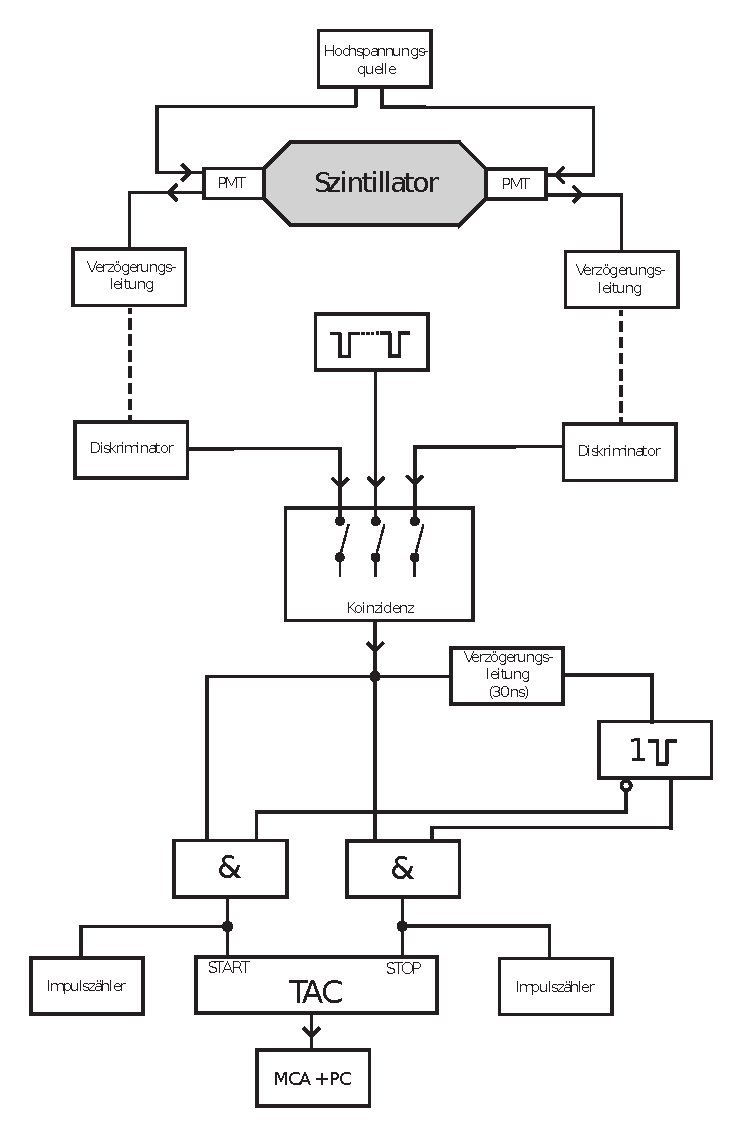
\includegraphics[width=0.8\textwidth]{pictures/schaltung.pdf}
    \caption{Blockschaltbild des Versuchsaufbaus \cite[3]{v01}.}
    \label{fig:schaltung}
\end{figure}


\subsubsection*{Photomultiplier}
Ein Photomultiplier (PMT) ist ein Detektor, der in der Teilchenphysik, 
der Astronomie und anderen Bereichen eingesetzt wird, um einzelne Photonen zu erfassen und zu verstärken. 
Bei der Messung der Lebensdauer kosmischer Myonen wird ein Photomultiplier (PMT) verwendet, 
um das Lichtsignal zu registrieren, das entsteht, 
wenn ein Myon in einem Szintillationsdetektor zerfällt. 

\subsubsection*{Szintillationsdetektor}
Ein Szintillator ist ein Detektor, der in der Lage ist, 
ionisierende Strahlung wie beispielsweise kosmische Strahlung zu detektieren. 

Es gibt verschiedene Arten von Szintillatoren wie organische und anorganische Szintillatoren,
die sich in ihrer Funktionsweise und ihrem Anwendungsgebiet unterscheiden.

Organische Szintillatoren bestehen aus einem organischen Material.
Die darin eindringenden Teilchen regen die Moleküle des Materials zu Schwingungen an. 
Nach Abgabe eines Photons gehen die angeregten Moleküle wieder in den Grundzustand über.
Der Vorteil dieses Material besteht deswegen in der Zeitauflösung, 
während eine Energieauflösung aufgrund der breiten Frequenzmodenverteilung benachteiligt ist.

Anorganische Szintillatoren bestehen aus anorganischen Materialien wie Kristallen oder Keramik. 
Dabei ionisiert sich das Material und erzeugt nach Aktivierung ein Lichtsignal.
Anders als beim organischen Material, liegen hier diskrete Ionisationsenerigen vor,
weswegen eine höhere Energieauflösung möglich ist.

\subsubsection*{Verzögerungsleitung}
Die Verzögerungsleitungen gleichen Unterschiede in der Signalübermittlung aus
und werden hier anpassbare bzw. zuschaltbare Kabel realisiert.

\subsubsection*{Diskriminator}
Das durch die Verzögerungsleitung gehende Signal wird durch Diskriminatoren geleitet.
Dabei wird das schwankende Signale der Photomultiplier ab einer gewissen Schwelle in diskrete
Ereignissignale umwandelt.

\subsubsection*{Koinzidenz}
Anschließend erreichen beide Signale eine Koinzidenzschaltung, welche ein Ausgangssignal
erzeugt, sobald zwei Photomultiplier gleichzeitig ein Signal aussenden.

